\startchapter{Automated Trojan Detection}
\label{chapter:trojanDetection}
\section{Methodology}
Figure~\ref{fig:Concept} provides a visual representation of the basic concept assumed for the purposes of this work. 
All stages of production of an \acrshort{FPGA} implementation are done "in-house" with the exception of the fabrication process. 
It is assumed that any trojan discovered is inserted in the fabrication phase; all other stages are trusted.  
The method of automated trojan detection described in this work would take place in the 'testing' phase of the life-cycle. 
\begin{figure}[h]
	\centering
	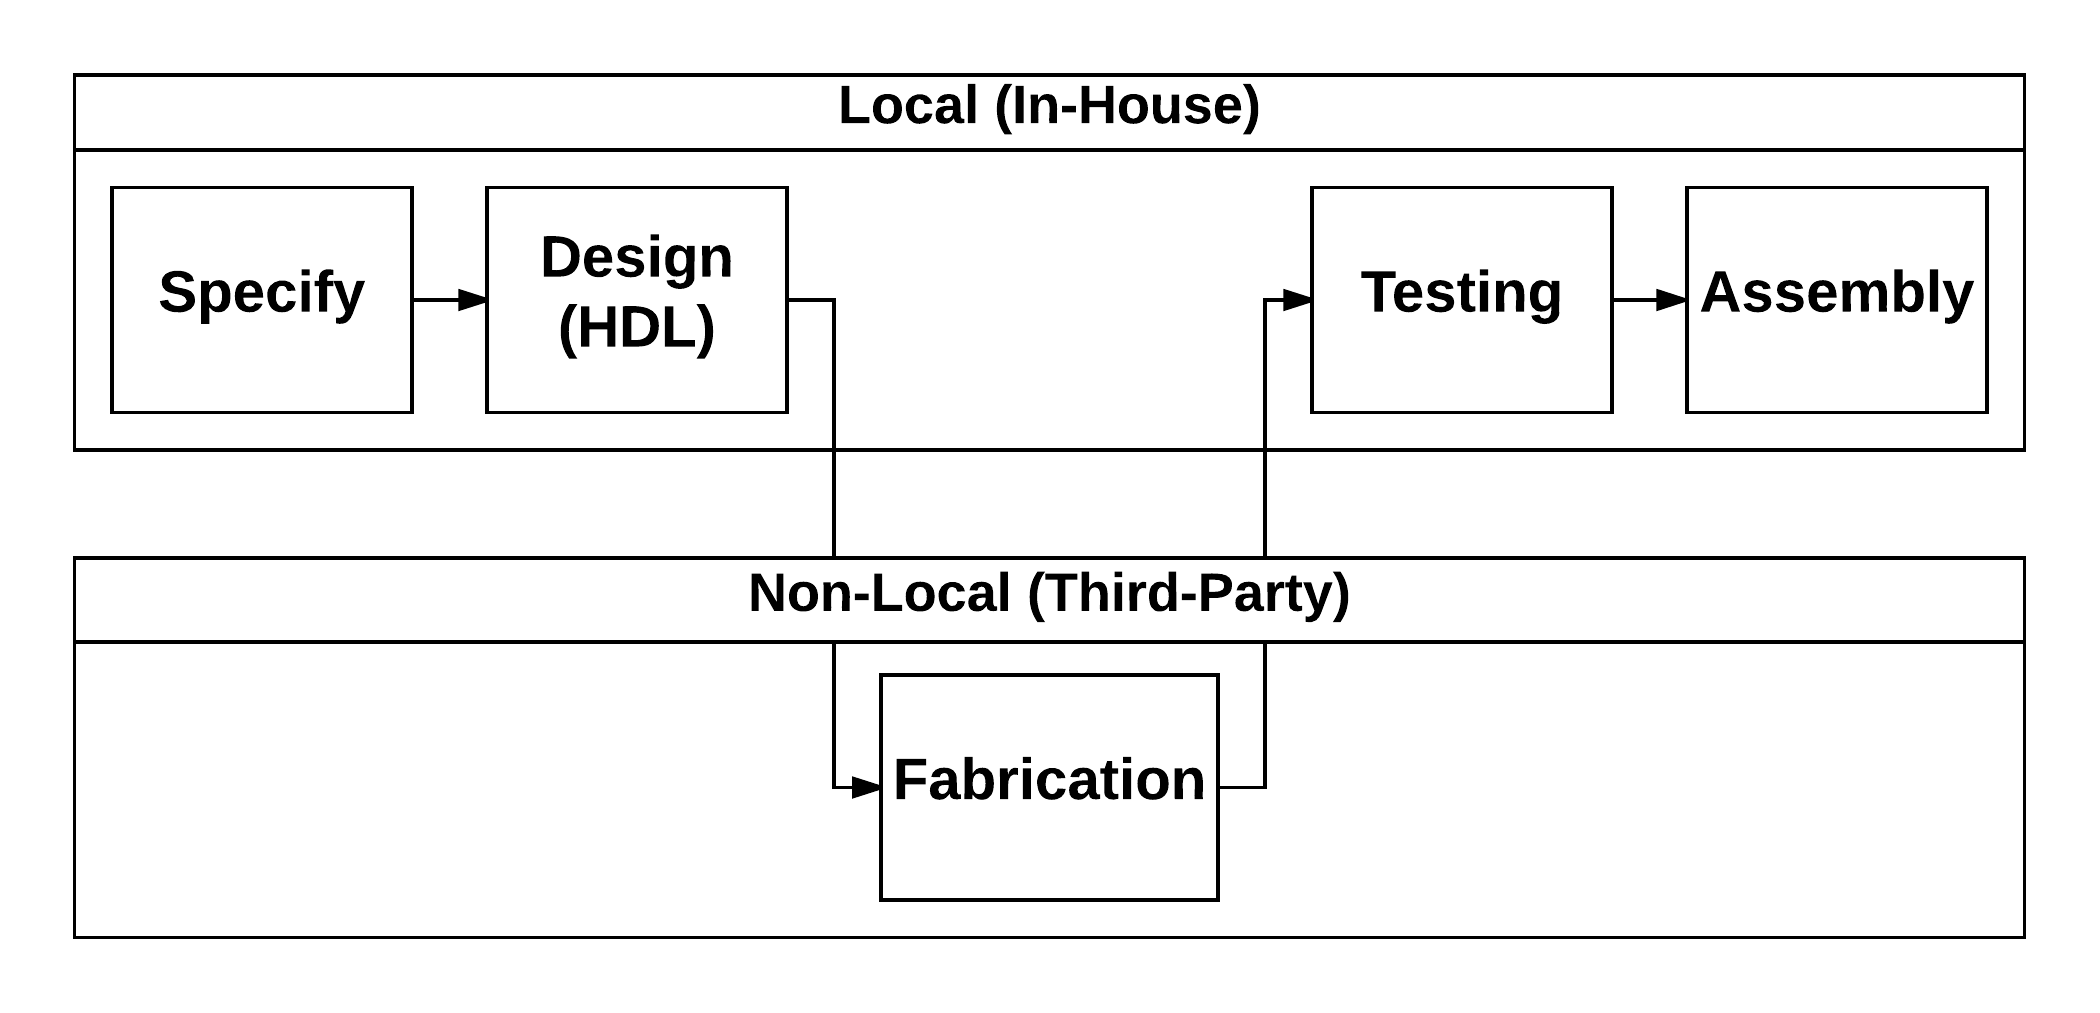
\includegraphics[width=1\linewidth]{figures/Concept}
	\caption[FPGA Life-Cycle]{FPGA Life-Cycle}
	\label{fig:Concept}
\end{figure}

Figure~\ref{fig:methodologyOverview} shows an overview of the trojan detection scheme.
\acrshort{FPGA} designs are written in a \acrfull{HDL}.
\Xilinx provides a series of \acrfull{UI} or command line tools to process the design known as the 'tool-chain'.
The tool chain generates a series of files that are used for a variety of purposes.
The Bit file is a binary representation of the design to be implemented.
It is referred to as the \gls{Bitstream} or Configuration \gls{Bitstream} and is the final form which is loaded into the device.
\begin{figure}
	\centering
	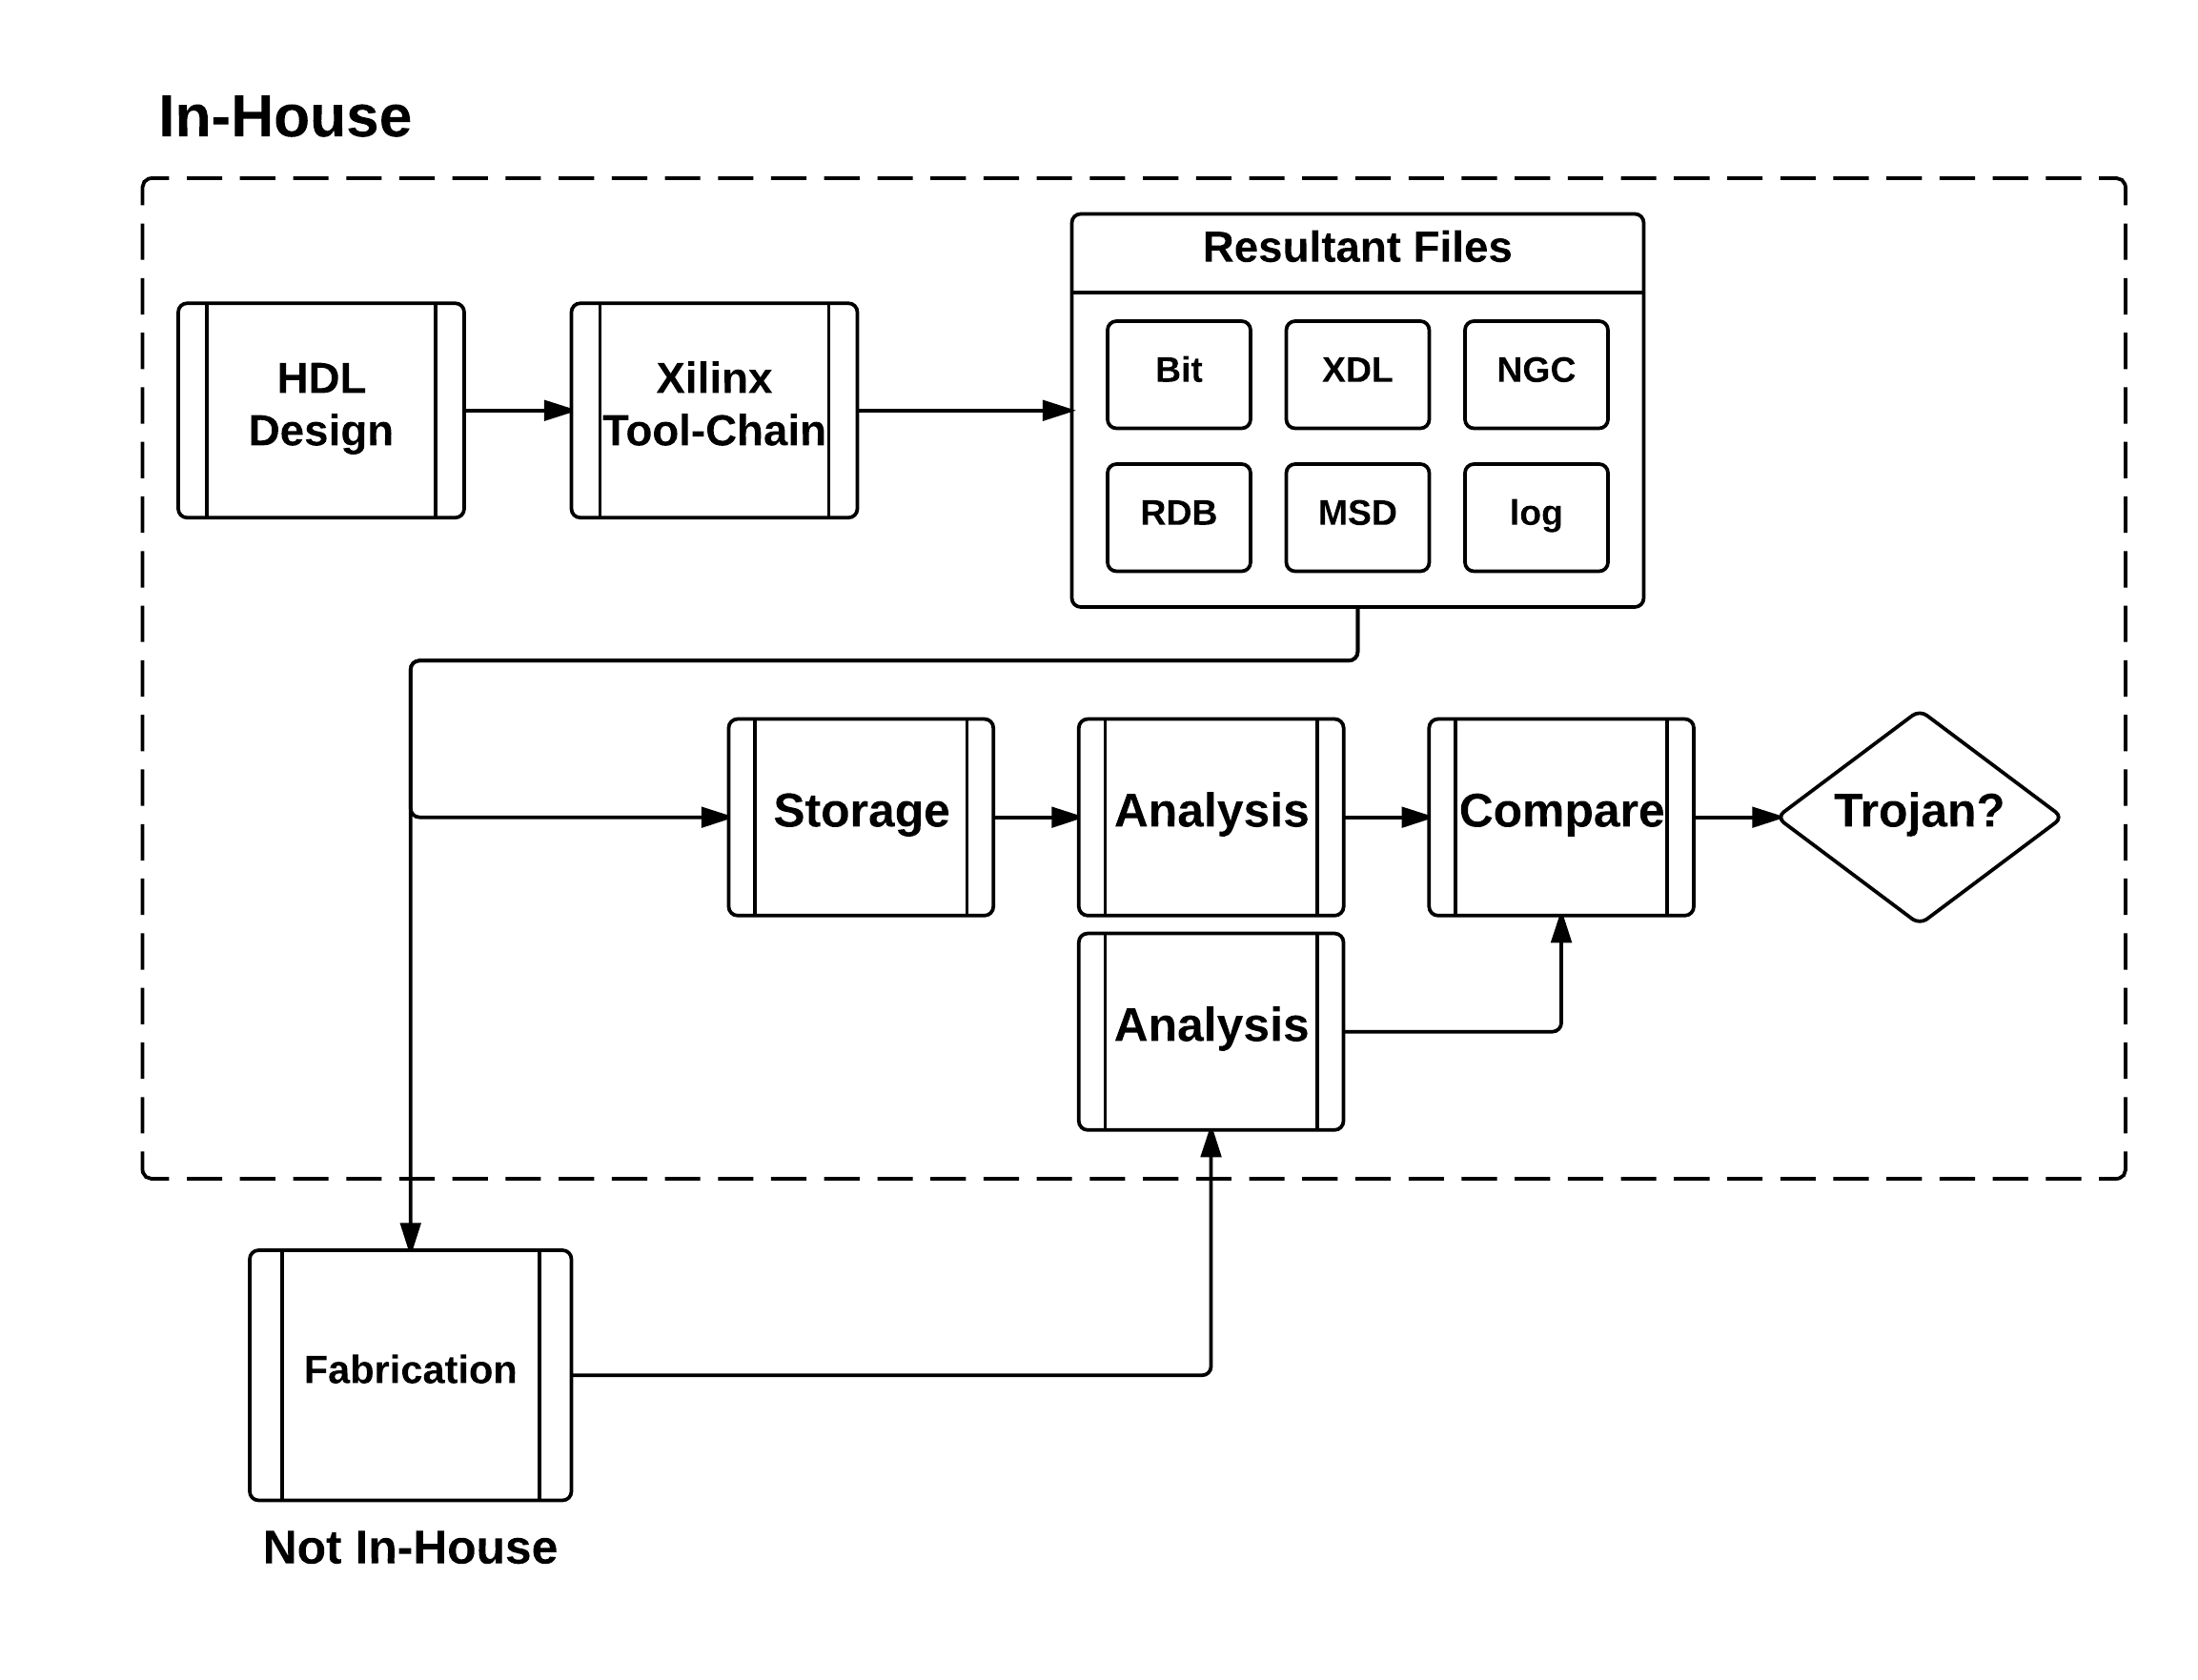
\includegraphics[width=1\linewidth]{Figures/methodologyOverview}
	\caption[Methodology Overview]{Methodology Overview}
	\label{fig:methodologyOverview}
\end{figure}
This Bit file is also one of the primary files sent to the fabrication house where it will be implemented onto the batch of devices ordered.
The resultant files are kept in secure storage while a copy is sent to be fabricated; these 'clean' copies are reffered to as \gls{golden}.
Though it is known that fabrication houses will often attempt to make optimizations on designs this methodology requires that no such efforts are made.
When the completed batch of fabricated chips are returned the \gls{Bitstream} is extracted via the method described in section~\ref{sec:bitstreamExtraction}. 
That which is extracted is referred to as the \gls{target} \gls{Bitstream}.
The \gls{golden} and \gls{target} \gls{Bitstream}s are analyzed in conjunction to detect differences, described in section~\ref{sec:fpgaBitStream}.
Any discovered differences are then attributed to the corresponding component in the architecture, described in section~\ref{sec:tileMapping}.
Finally, descriptive attributes presented in section~\ref{sec:topology} are returned to the user, described in section~\ref{sec:trojanAttributes}. 

\section{FPGA Architecture and Configuration} \label{sec:architectureAndConfig}
A \Xilinx \acrfull{FPGA} is comprised of a matrix of blocks referred to as the 'gate-array' and is shown in Figure~\ref{fig:FPGA}.
A device can contain anywhere from a couple hundred to a few thousand blocks; they are arranged into columns by type.
A block will consist of one or multiple tiles depending on the type.
A tile is a component specific to a particular function such as \acrfull{IO}, design logic, memory...etc but their detailed functionality can be configured by the user.
An \acrshort{FPGA} may have over one-hundred different types of tiles however each column is comprised entirely by a single block type.
Columns are separated by clock regions as shown by the dashed lines in Figure~\ref{fig:FPGA}.
Each region is an independent array of blocks that uses a dedicated clock resource; this minimizes clock skew from causing undesired timing delays.
\begin{figure}[h]
	\centering
	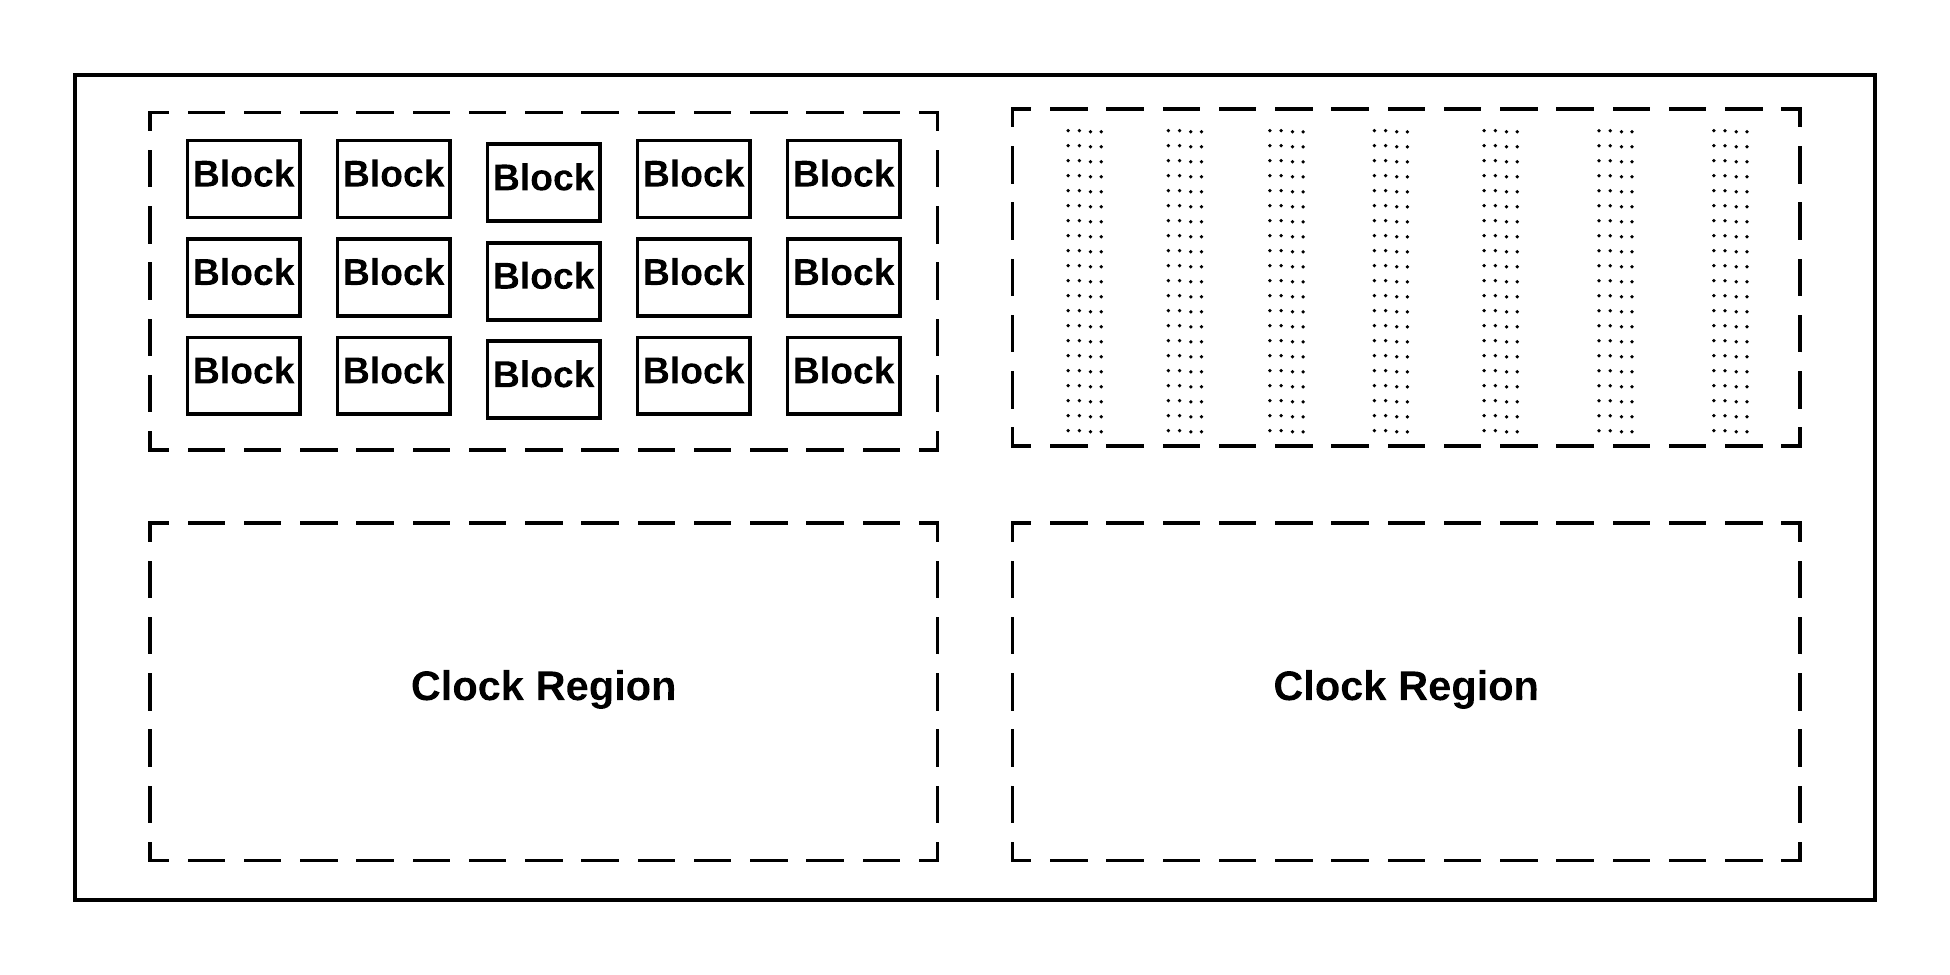
\includegraphics[width=1\linewidth]{figures/FPGA}
	\caption[Rudimentary Layout of a Virtex Gate-Array]{Rudimentary Layout of a Virtex Gate-Array}
	\label{fig:FPGA}
\end{figure}
Though each tile has a designated purposes (ex. \acrfull{IO}, \acrfull{CL}, memory...etc) their functionality can be configured by the user; this is how designs are implemented on a device.
The configuration of each tile is dictated by the \gls{Bitstream}. 
To improve performance the contents of the gate-array is referred to as dynamic.
A dynamic device is unable to retain the contents of its memory when it looses power.
To prevent having to plug in a device and download the configuration every time it is powered on, an external static memory device (i.e. retains its contents with loss of power) holds the \gls{Bitstream}. 
When an \acrshort{FPGA} is powered on the \gls{Bitstream} is loaded from the external memory (often \acrfull{SRAM}) into the gate-array, as can be seen in Figure~\ref{fig:architecture}.

\begin{figure}
\centering
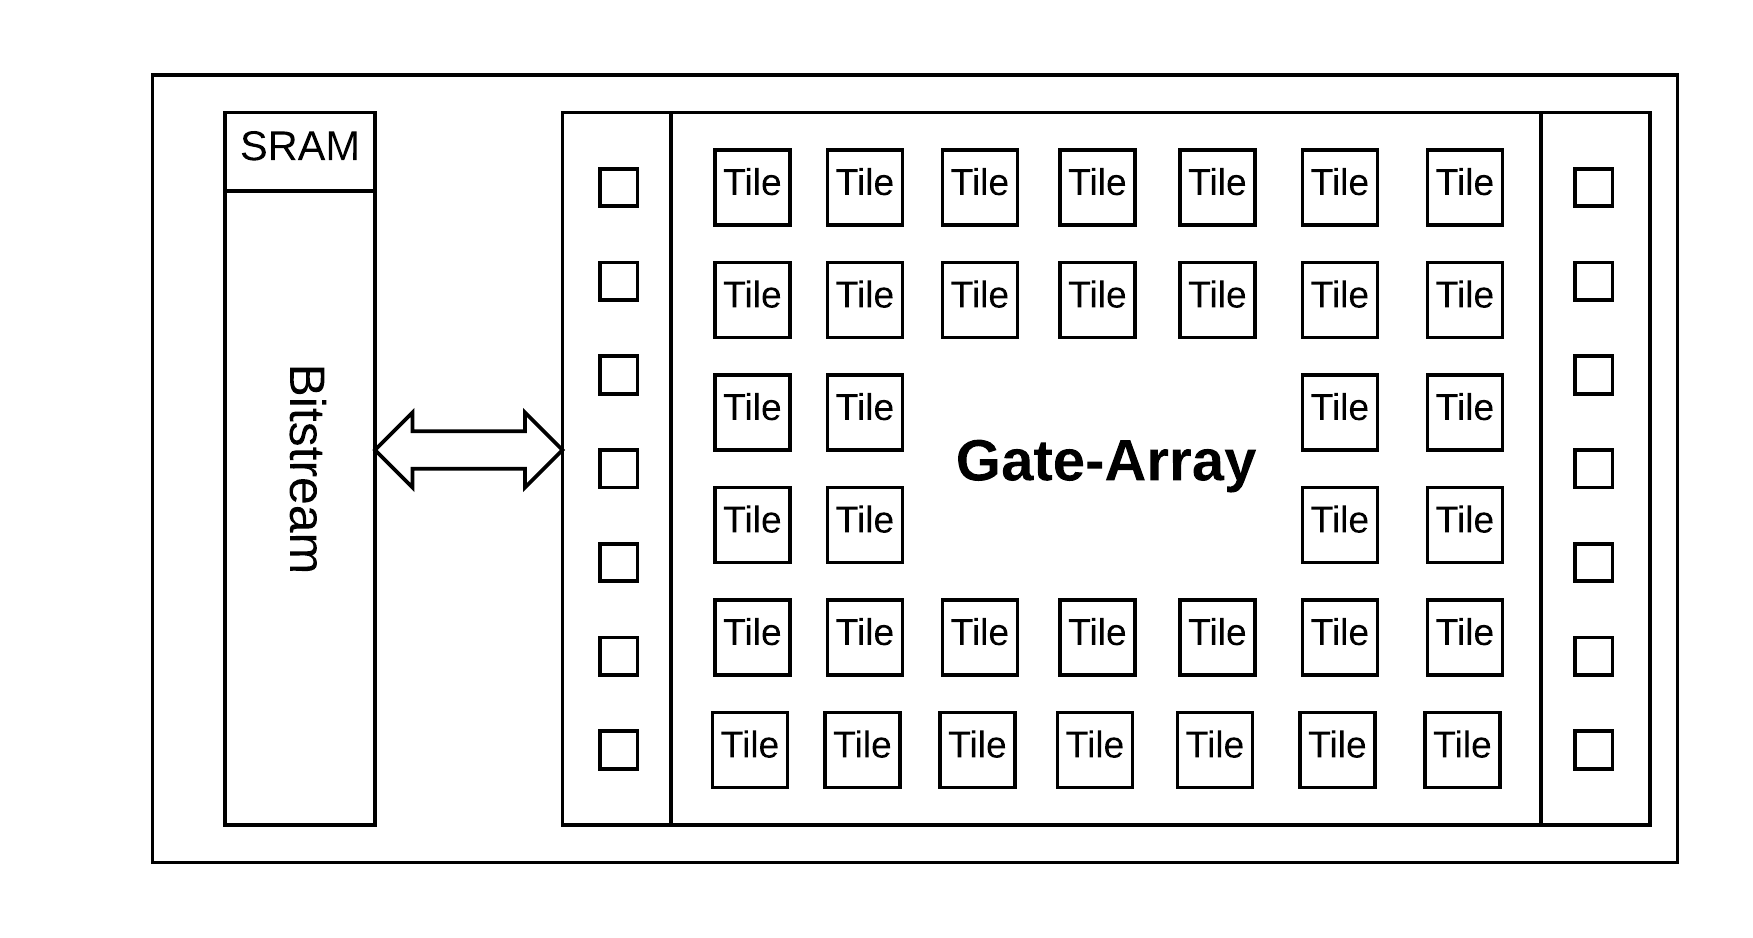
\includegraphics[width=0.9\linewidth]{Figures/architecture}
\caption[FPGA Device Layout]{FPGA Device Layout}
\label{fig:architecture}
\end{figure}

\section{\gls{Bitstream} Extraction} \label{sec:bitstreamExtraction}
In order to detect any trojans in the \gls{target} device the configuration \gls{Bitstream} will need to be recovered.
As mentioned in section~\ref{sec:architectureAndConfig} the \gls{Bitstream} is stored in a memory unit external to the gate-array.
All \Xilinx devices provide a feature known as \gls{Readback}.
There are two styles of \gls{Readback}; \gls{Readback} verify and \gls{Readback} Capture.
The \gls{Readback} capture method provides a large quantity of debug information which is not needed; \gls{Readback} verify will be used.
\gls{Readback} verify is the process where the device is put into a 'frozen' state during run-time and all of the configuration bits are returned from the gate-array to the \acrshort{SRAM}. 
The results can then be uploaded to a \acrfull{PC} for analysis.
This process overwrites the original frame data in the \acrshort{SRAM} with the values which actually configured the device. 
By using this method rather than simply reading the \acrshort{SRAM} it ensures that what is tested in section~\ref{sec:fpgaBitStream} is actually what configured the device.
This minimizes risk of tampered external memory units or configuration mechanics. 

\section{The \acrshort{FPGA} \gls{Bitstream} Analysis} \label{sec:fpgaBitStream}
The \Xilinx \gls{Bitstream} is a binary file composed of a series of 32-bit words organized into 'frames'.
A frame is a string of single bits that span from the top to the bottom of a clock region of a device as seen in the top-right quadrant of Figure~\ref{fig:FPGA}.
A frame affects every block in a column and multiple horizontally adjacent frames are required to configure an entire column.
Each frame is uniquely identified by a 32-bit address and is the smallest addressable element.
The composition of the frame address is fairly consistent across the \Xilinx catalog however there are small differences between device families.
The following is the structure of the Virtex-5 family frame address scheme according to~\cite{virtex5ConfigGuide}.
The make-up of a frame address is shown in Table~\ref{tbl:frameAddress}.
\begin{table}[h]
	\centering
	\caption{Frame Address}
	\label{tbl:frameAddress}
	\resizebox{\textwidth}{!}{
		\begin{tabular}{|c|c|c|c|c|c|c|c|c|c|c|c|c|c|c|c|c|c|c|c|c|c|c|c|c|c|c|c|c|c|c|c|}
			\hline
			\multicolumn{8}{|c|}{Unused} & \multicolumn{3}{c|}{BA} & T & \multicolumn{5}{c|}{Row Address} & \multicolumn{8}{c|}{Major Address} & \multicolumn{7}{c|}{Minor Address} \\ \hline
			31 & 30 & 29 & 28 & 27 & 26 & 25 & 24 & 23 & 22 & 21 & 20 & 19 & 18 & 17 & 16 & 15 & 14 & 13 & 12 & 11 & 10 & 9 & 8 & 7 & 6 & 5 & 4 & 3 & 2 & 1 & 0 \\ \hline
			0 & 0 & 0 & 0 & 0 & x & x & x & x & x & x & x & x & x & x & x & x & x & x & x & x & x & x & 0 & 0 & 0 & 0 & 0 & 0 & 0 & 0 & 0 \\ \hline
		\end{tabular}		
	}
\end{table}
The \acrfull{BA} identifies the block type.
\begin{itemize}
	\item BA 0: Logic type.
	\item BA 1: \acrfull{BRAM}.
	\item BA 2: \acrshort{BRAM} Interconnect.
	\item BA 3: \acrshort{BRAM} non-configuration frame.
\end{itemize}
The logic block contains the columns which provides the primary configuration for the device (\acrshort{CLBs}, \acrshort{IOBs}... etc).
The \acrshort{BRAM} columns initialize the memory for the device while the \acrshort{BRAM} Interconnect columns configure how the logic of the design interacts with the \acrshort{BRAM}.

In the case of the Virtex-5 family each clock region is composed of twenty blocks in a column separated by a horizontal clock bus as shown in Figure~\ref{fig:RowOrder}.
\begin{figure}[h]
\centering
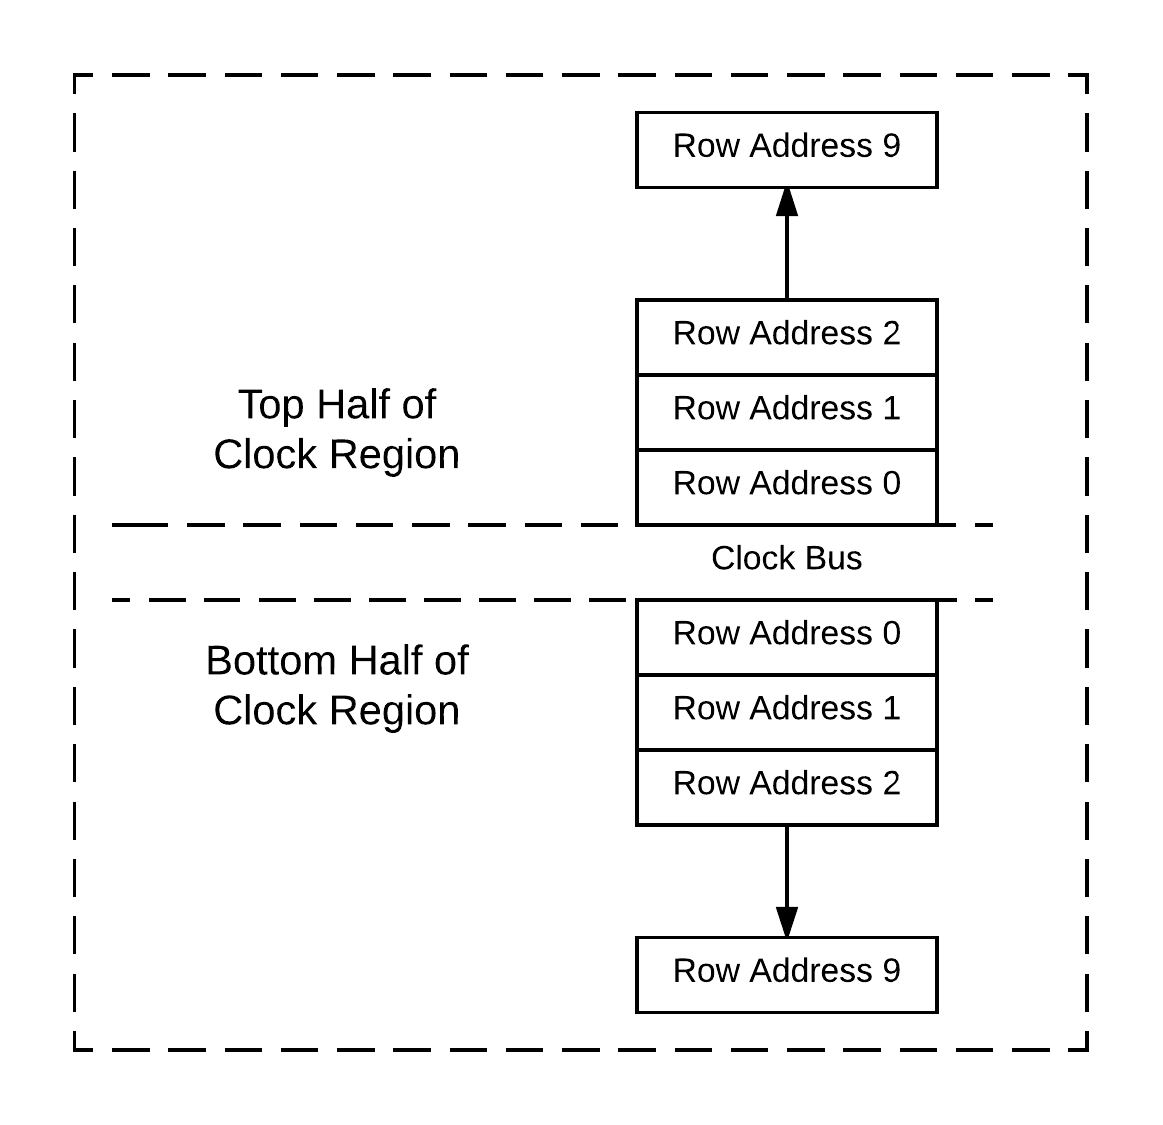
\includegraphics[width=.7\linewidth]{Figures/RowOrder}
\caption[Row Order of Virtex-5 Clock Region]{Row Order of Virtex-5 Clock Region}
\label{fig:RowOrder}
\end{figure}
Each row of blocks is given a row value in it's address that increments away from the clock bus starting at 0. 
The frame address includes a Top indicator bit in position 20 that indicates whether the specified row is above or below the horizontal clock bus.
The major address specifies the block within the row.
These addresses are numbered from left to right and begin at 0.
The minor address indicates the frame number within a column. 
Table~\ref{tbl:minorAddressNumbers} provides the number of frames per column type.
\begin{table}[]
	\centering
	\caption{Number of Frames (minor addresses) per Column}
	\label{tbl:minorAddressNumbers}
	\begin{tabular}{|c|c|}
		\hline
		Block             & Number Of Frames \\ \hline
		CLB               & 36               \\ \hline
		DSP               & 28               \\ \hline
		\acrshort{BRAM} & 30               \\ \hline
		IOB               & 54               \\ \hline
		Clock             & 4                \\ \hline
	\end{tabular}
\end{table}
The number of frames given in Table~\ref{tbl:minorAddressNumbers} corresponds to the block in the column.
As described in section~\ref{sec:architectureAndConfig} a block may contain multiple tiles.
In a CLB column a block consists of an interconnect tile, also known as a \acrfull{SM} and a \acrshort{CLB}.
To further understand how frames configure tiles a mapping must be made between each frame and the corresponding tile.
This is described in section~\ref{sec:tileMapping}.

\section{Tile Mapping} \label{sec:tileMapping}
In the case of Virtex-5 devices a frame is composed of 41 words that can be thought of as a vertical stack that aligns with the column it configures.
As described in section~\ref{sec:fpgaBitStream} a row consists of a stack of basic blocks; there are 20 \acrshort{CLB} blocks per column, 40 \acrshort{IOB}s, 4 \acrshort{BRAM}...etc.
\begin{figure}[h]
	\centering
	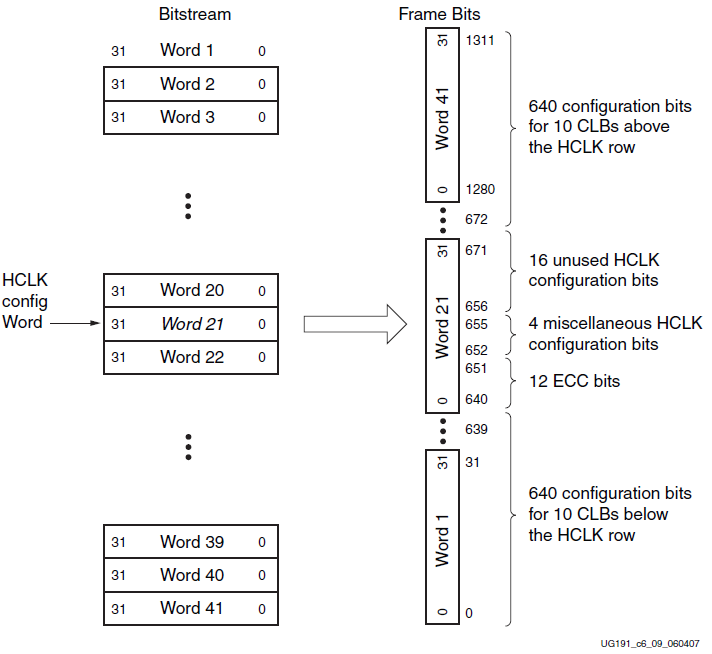
\includegraphics[width=0.9\linewidth]{Figures/frameTileMap}
	\caption[Configuration Words in the Bitstream~\cite{virtex5ConfigGuide}]{Configuration Words in the Bitstream~\cite{virtex5ConfigGuide}}
	\label{fig:frameTileMap}
\end{figure}
As can be seen in Figure~\ref{fig:frameTileMap} the central word in a frame configures the horizontally running clock bus.
The remaining words are used to configure the blocks in the column.
From this, equation~\ref{eqn:numWordsPerBlock} can be deduced which is used to compute the number of 32-bit words that span each block.
\begin{equation} \label{eqn:numWordsPerBlock}
n = (W - C) + B
\end{equation}
where:
\begin{conditions}
	n     &  Number of Words per Block \\
	W     &  Number of 32-bit words per frame \\   
	C     &  Number of clock words per frame \\
	B     &  Number of blocks per column
\end{conditions}
As shown in Figure~\ref{fig:frameTileMap} words are addressed from the 'top' of a device downwards.

\begin{equation} \label{eqn:getTileNumber}
i = n - \floor*{w / B}
\end{equation}
where:
\begin{conditions}
	i     &  Word Number in frame\\
	n     &  Number of Words per Block \\
	$w$   &  Number of 32-bit words per frame \\  
	B     &  Number of blocks per column
\end{conditions}

\section{Trojan Attributes} \label{sec:trojanAttributes}



%This is where you go all out and tell us all about your new discovery and research related to the problem in the previous chapter. No arrogant sweeping statements which cannot be fully justified, but no false modesty either. You must impress your reader that you have accomplished something.
%
%Simply summarized, this chapter should be comprised of at least two main sections, each with appropriate subsections. The first section should describe:
%\begin{itemize}
%\item {what the new approach is;}
%\item {what is really totally new;}
%\item {what is incrementally new;}
%\item {what you built upon.}
%\end{itemize}
%
%The second part should describe fully how the new approach works, both with the overall theoretical exposition (e.g. an algorithm) and with as many examples as necessary for clarity. Remember that if the reader does not understand fully, you will get a lot of questions and doubts. Good examples, good figures, good diagrams with super clear tutorial explanations can be a joy to read and make even a small contribution appear to be more impressive. Are you afraid that if you are too tutorial your work will not seem as deep and difficult? Only shallow people will make such a superficial evaluation, have trust instead in the wisdom of your supervisory committee.
%
%Use at least one good example throughout, and even better if this is one of the examples you used in Chapter 2 to describe the original problem.
%
%By the way, this would be the first chapter I would write. This is what I know best right now, as I just finished working on it. It is clear to me and on the tip of my fingers. Start with your strengths! The second chapter I would write is the next one about the experiments, followed closely by chapter 2 describing the problem. It may not seem intuitive to you, but it works and it is the most productive way I ever found to finish a document.
%
%
%\input chapters/3/sec_latexhelp
